%%%%%%%%%%%%%%%%%%%%%%%%%%%%%%%%%%%%%%%%%
% Journal Article
% LaTeX Template
% Version 1.3 (9/9/13)
%
% This template has been downloaded from:
% http://www.LaTeXTemplates.com
%
% Original author:
% Frits Wenneker (http://www.howtotex.com)
%
% License:
% CC BY-NC-SA 3.0 (http://creativecommons.org/licenses/by-nc-sa/3.0/)
%
%%%%%%%%%%%%%%%%%%%%%%%%%%%%%%%%%%%%%%%%%

%----------------------------------------------------------------------------------------
%	PACKAGES AND OTHER DOCUMENT CONFIGURATIONS
%----------------------------------------------------------------------------------------

\documentclass{IOS-Book-Article}
\usepackage{amsmath}
\usepackage{booktabs,array}
\newcolumntype{A}{@{}llccc >{$} r <{$} @{} >{${}} l <{$}@{}}
\usepackage{fancyhdr}

\usepackage{lipsum} % Package to generate dummy text throughout this template
\usepackage{graphicx}
\usepackage[sc]{mathpazo} % Use the Palatino font
\usepackage[T1]{fontenc} % Use 8-bit encoding that has 256 glyphs
\linespread{1.05} % Line spacing - Palatino needs more space between lines
\usepackage{microtype} % Slightly tweak font spacing for aesthetics

%\usepackage[hmarginratio=1:1,top=32mm,columnsep=20pt]{geometry} % Document margins
\usepackage{multicol} % Used for the two-column layout of the document
\usepackage[hang, small,labelfont=bf,up,textfont=it,up]{caption} % Custom captions under/above floats in tables or figures
\usepackage{booktabs} % Horizontal rules in tables
\usepackage{float} % Required for tables and figures in the multi-column environment - they need to be placed in specific locations with the [H] (e.g. \begin{table}[H])
\usepackage{hyperref} % For hyperlinks in the PDF

\usepackage{lettrine} % The lettrine is the first enlarged letter at the beginning of the text
\usepackage{paralist} % Used for the compactitem environment which makes bullet points with less space between them

\usepackage{listings}

%\usepackage{abstract} % Allows abstract customization
%\renewcommand{\abstractnamefont}{\normalfont\bfseries} % Set the "Abstract" text to bold
%\renewcommand{\abstracttextfont}{\normalfont\small\itshape} % Set the abstract itself to small italic text

\usepackage{pdfpages}

%[doi=false,issn=false,url=false,language=false, keywords=false]
\usepackage{natbib}
%\usepackage{titlesec} % Allows customization of titles
%\renewcommand\thesection{\Roman{section}} % Roman numerals for the sections
%\renewcommand\thesubsection{\Roman{subsection}} % Roman numerals for subsections
%\titleformat{\section}[block]{\large\scshape\centering}{\thesection.}{1em}{} % Change the look of the section titles
%\titleformat{\subsection}[block]{\large}{\thesubsection.}{1em}{} % Change the look of the section titles

%\usepackage{fancyhdr} % Headers and footers
%\pagestyle{fancy} % All pages have headers and footers
%\fancyhead{} % Blank out the default header
%\fancyfoot{} % Blank out the default footer
%\fancyhead[C]{Running title $\bullet$ November 2012 $\bullet$ Vol. XXI, No. 1} % Custom header text
%\fancyfoot[RO,LE]{\thepage} % Custom footer text
\usepackage{color}
\newcommand{\mads}[1]{\textcolor{red}{[MadsR: #1]}}
\newcommand{\bjarke}[1]{\textcolor{red}{[Bjarke: #1]}}
\newcommand{\anders}[1]{\textcolor{red}{[Anders: #1]}}
\newcommand{\mathias}[1]{\textcolor{red}{[Mathias: #1]}}

\begin{document}
%----------------------------------------------------------------------------------------
%	TITLE SECTION
%----------------------------------------------------------------------------------------

\newpage

\pagestyle{plain}
%\def\thepage{}
\setcounter{page}{1}

\begin{frontmatter}    

\title{Programming Paradigms project 1: \\ A list based calendar}

\author{\fnms{Bjarke Thorn} \snm{Carstens} (bcarst09@student.aau.dk), studentnr. 20093648}, %

\address{Department of Computer Science, Aalborg University, Denmark}
%----------------------------------------------------------------------------------------


%\maketitle % Insert title

%\thispagestyle{fancy} % All pages have headers and footers

%----------------------------------------------------------------------------------------
%	ABSTRACT
%----------------------------------------------------------------------------------------

\begin{keyword}
Functional programming \sep Scheme \sep Calendar system
\end{keyword}
\end{frontmatter}

%----------------------------------------------------------------------------------------
%	ARTICLE CONTENTS
%----------------------------------------------------------------------------------------

%\begin{multicols}{2} % Two-column layout throughout the main article text

\section{Introduction} \label{sec:introduction}
I have written a program for constructing a simple calendar in scheme that I have named: \textbf{A list based calendar}, which will be referred to by the acronym \textbf{ALBC}. 
This report split up in different sections such that: \autoref{sec:internalrepresentations} explains the details regarding the internal representations of the \textbf{ALBC}. \autoref{sec:functionality} explains the overall functionality of the \textbf{ALBC} system and later goes into depth with specifics regarding the functionality of the system. \autoref{sec:reflection} details reflections regarding the assignment, and finally \autoref{sec:userguide} introduces a short user guide for the testing \textbf{ALBC}. 


\section{Internal representations} \label{sec:internalrepresentations}
This section will explain the details regarding the internal representations used in \textbf{ALBC} for calendars, appointments and time. Furthermore the system includes getters for accessing appointment and time lists.

\subsection{Calendar}
The representation of a calendar in \textbf{ALBC} is a list that always starts with the string identifier "calendar" as the first index. The rest of the indices can then consist of either calendars or appointments, though there is no actual checks that ensure this, which would have been ideal. One way to perform the checks would be to simply check on the first index when including calendars, and to include a similar identifier into appointment representation to identify appointments in similar fasion. An example of a simple calendar containing only appointments can be seen in \autoref{code:calendarRepresentation} below. \\

\begin{lstlisting}[frame=single, caption={Calendar representation}, label={code:calendarRepresentation}] 

'("calendar"
  ((2005 11 24 23 55) (2005 11 24 23 56) "my content1")
  ((2005 11 24 23 55) (2005 11 24 23 56) "my content2")
  ((2005 11 24 15 55) (2005 11 24 16 54) "my content3")
  ((2005 11 24 11 55) (2005 11 24 13 54) "my content4")
  ((2005 11 24 15 55) (2005 11 24 16 54) "my content5")
  ((2005 11 24 11 55) (2005 11 24 13 54) "my content6")
  ((2005 11 24 11 55) (2005 11 24 13 56) "my content7"))
\end{lstlisting}

\subsection{Appointment}
Appointments in system are represented by a list of size 3, where the first interval in the startTime, the second interval the endTime and the third interval, the text content of the appointment. Also, as previously mentioned, an appointment sadly has no unique identifier to easily identify it. A new appointment is constructed by the function \textbf{(createAppointment startTime endTime content)} see \autoref{code:appointmentCreation}, and \autoref{code:appointmentRepresentation} for the resulting list representation.

\begin{lstlisting}[frame=single, caption={Creating an appointment}, label={code:appointmentCreation}] 
(createAppointment 
	(createTime 2005 11 24 23 55)
	(createTime 2005 11 24 23 56) 
	"my content2")
\end{lstlisting}

\begin{lstlisting}[frame=single, caption={Appointment representation}, label={code:appointmentRepresentation}] 
'((2005 11 24 23 55) (2005 11 24 23 56) "my content2")
\end{lstlisting}

When creating an appointment with \textbf{(createAppointment startTime endTime content)} the function ensures the following, or returns an error in case any of the conditions fail:
\begin{itemize}
\item The startTime is before the endTime, this check is assisted by a function \textbf{(calcTimeSeconds time)} that converts each of \textit{time} list to seconds before a comparison is performed.
\item The date, startTime and endTime, of the appointment takes place on one day. This means that the dates of start- and endTime are on the same day, month, and on the same year.
\end{itemize}


\subsection{Time}
The representation of time in \textbf{ALBC} is a list of (year month day hour minute), where all elements are represented by integers, an example of this is: \textbf{(2005 11 24 23 56)}. A \textit{time} list is create by the function \textbf{(createTime year month day hour minute)}, see \autoref{code:createTime} below.

\begin{lstlisting}[frame=single, caption={Definition of (createTime year month day hour minute)}, label={code:createTime}]  % Start your code-block

(define createTime (lambda(year month day hour minute)
 	(list (checkYear year) 
 		(checkMonth month) 
 		(checkDay day) 
	 	(checkHour hour) 
	 	(checkMinute minute))))  
\end{lstlisting}

When creating a \textit{time} list, the \textbf{checkYear, checkMonth, checkDay, checkHour and checkMinutes} functions ensure the following for the time format is well formed meaning that: The Provided year is bigger than 0, month is between 1-12, day is between 1-31, hour is between 0-23 and minute is between 0-59.

\section{Functionality} \label{sec:functionality}
\textbf{ALBC} provides functionality for creating a root calendar containing calendars and/or appointments. It is possible to add, and delete, calendar and appointments to the root calendar, and the root calendar can also be flattened such that nested appointments are placed into a single root calendar consisting only of appointments. 
\textbf{ALBC} also provides functionality for presenting the appointments in a calendar within a html table. It can find appointments in a given calendar, based on a fitting predicate specified by the user, as well as return only the earliest or latest appointment in a calendar based on a user specified time interval. This functionality and more is provided by the following functions: 

\begin{itemize}
\item \textbf{(addAppointmentToCalendar cal apt)} : simply adds the provided appointment to the end of the provided calendar.
\item \textbf{(deleteAppointmentFromCalendar cal apt)} : deletes the appointment \textit{apt} only from the root calendar \textit{cal}, ideally it could be made recursively. 
\item \textbf{(deleteCalendarFromCalendar cal delCal)} : deletes the calendar \textit{delCal} only from the root calendar, ideally it could be made recursively. Unlike the implementation of \textbf{deleteAppointmentFromCalendar} this function simply uses \textbf{equal?} to compare the calendars.
\end{itemize}

The following functions provide functionality for presentation and filtering of calendars and appointments in \textbf{ALBC}:
\begin{itemize}
\item \textbf{(flatten-calendar cal)} : simply flattens the provided calendar, such that a calendar only including the appointments of the original calendar is returned, with the exception of the first index which always holds the string "calendar".
\item \textbf{(parseCalendar cal res)} : works the same way as \textbf{flatten-calendar} except that the resulting calendar only holds appointments. 
\item \textbf{(present-calendar-html cal from-time to-time)} : returns html that shows a table including all appointments that take place in the provided time-interval of from-time to to-time. Both the start time and end time of an appointment has to be within the interval. An example of the output can be seen in the appendix see \autoref{sec:generatedhtml}.
\item \textbf{(find-appointments cal pred)} : returns all appointments in cal that satisfies the predicate \textit{pred}.
\item \textbf{(find-first-appointment cal pred)} : returns only the earliest appointment, based on startTime, that satisfies the predicate \textit{pred}. In case of identical appointments, the first appointment is kept.
\item \textbf{(find-last-appointment cal pred)} : returns only the latest appointment, based on startTime, that satisfies the predicate \textit{pred}. Does the opposite of \textbf{find-first-appointment} in case of identical appointments, and thus replaces the previous appointment.
\item \textbf{(appointments-overlap? ap1 ap2)} : returns true if the time of provided appointments overlap.
\item \textbf{(calendars-overlap? cal1 cal2)} : returns true if the provide calendars have appointments that overlap in time.
\end{itemize}



\section{Reflection} \label{sec:reflection}
I didn't get to finish the program to the point that I had wished for. Mainly I had the hope being able to finish a function for generating a html calendar presented in a proper weekly format. Also not including an identifier in my appointments early made me not wanting to spend time refactoring it, otherwise this is one of the first things I would change as it could be changed rather easily. More format checking on the internal representations would also have been an easy next step. It could also be considered the functions \textbf{find-last-appointment} and \textbf{find-first-appointment} should be able to return multiple appointments in case of appointments with equal time.

\subsection*{Static typing vs dynamic typing}
I actually didn't pay much attention to the dynamic typing of scheme, though in a way it was nice not having to worry about  being explicit with types. Especially because there are plenty of other aspects to use your attention on, and think about, when programming scheme. I never really had any point where type was an issue.

\subsection*{Functional vs object-oriented paradigm}
The leap from the object-oriented paradigm was rather big, with my currently experience structuring a program, for a specific domain, in OOP is a lot easier. Especially learning to use recursion properly hasn't exactly been a walk in the park. My impression is that the success of using it properly is very dependent on avoiding complexity, especially by being able to keep functions small and decomposed properly. Most of all this has been an issue while trying to generate proper formed html. In this context one of the bigger issues was keeping track of state, in a sense it's nice to avoid assignment since recursion could become a nightmare with it. Though on the other hand trying to keep track of state through recursion in a function parameters wasn't always easy to me. 
Another aspect that has been quite different is the issue of encapsulation and internal representation. Working with lists hasn't been much of an issue, however I didn't properly consider the issue of being able to identify my appointments, other than checking for complete equality of the entire list.

One thing I'm not looking forward to is using scheme has a language for a bigger code bases, as it already becomes a little difficult for me to manage it with around 500 lines of code. Obviously this aspect may greatly improve with more experience and learning of best practices. Though to me it seems that the functional paradigm does require a bit more of the programmer. Though I'm looking forward to getting familiar with either scala or F\# in the future.

\subsection*{Higher order functions}
I didn't make particularly much use of higher order functions, which could probably have been quite useful. Though one of the cases where I did use it was for the different variations of \textbf{(find-appointments cal pred)}, which was neat even though the most attractive filter I can think of is getting appointments within a specific time-interval or with a specific text content.   

\section{User guide for ALBC} \label{sec:userguide}
The attached program file contains quite a bit of commented out test code, from line 355-481, which can easily be used for testing the various functions defined. It also includes 4 predefined calendars named: "cal1", "cal2", "cal3" and "cal4", which may come in handy when testing. The last part of the file from line 484 is unfinished code that was the start of trying to generate the week based html calendar.


\section{Appendix}
\begin{figure}
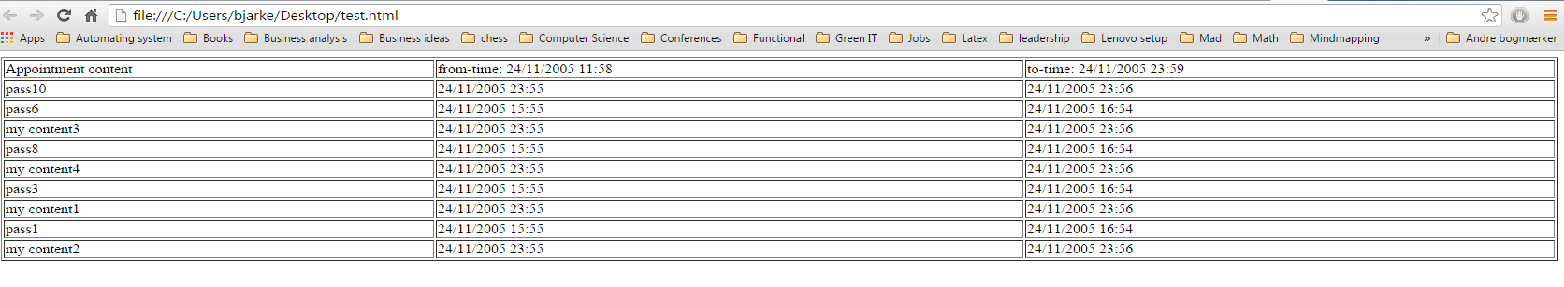
\includegraphics[scale=0.4]{./pic.png}
\label{sec:generatedhtml}
\caption{Generated html}
\end{figure}


%----------------------------------------------------------------------------------------
%	REFERENCE LIST
%----------------------------------------------------------------------------------------

%\bibliographystyle{plainnat}



%\begin{thebibliography}{99} % Bibliography - this is intentionally simple in this template

%\bibitem[Figueredo and Wolf, 2009]{Figueredo:2009dg}
%Figueredo, A.~J. and Wolf, P. S.~A. (2009).
%\newblock Assortative pairing and life history strategy - a cross-cultural
 % study.
%\newblock {\em Human Nature}, 20:317--330.
 
%\end{thebibliography}

%----------------------------------------------------------------------------------------

%\end{multicols}

\end{document}